\section{Hardware}

\subsection{Akkus und Ladegerät}
Die Akkus die wir benutzen sind 2-Zellen Litium-Polymer-Akkus mit 950mAh Kapazität.
Zum Laden müssen die Akkus mit beiden Steckern mit dem Ladegerät verbunden werden, danach kann man mit dem LiPo-Balance-Programm die Akkus laden.
Wichtig ist, dass im Ladegerät 2S ausgewählt ist und die Stromstärke nicht über 2A eingestellt wird.
(mit 1A Stromstärke zu laden ist schonender für die Akkus, über 4A können die Akkus anfangen zu brennen)
Die Akkus sollten nicht ohne Aufsicht geladen werden.

Am Quadrocopter wird der Akku mit dem JST-Connector angeschlosse. Die Spannungsüberwachung ist intern angeschlossen.

Um neue Firmware zu flashen muss der Quadrocopter über USB mit dem Rechner verbunden werden, der Akku sollte dabei nicht angeschlossen sein, um ein unkontrolliertes Loslaufen der Motoren zu verhindern.

\subsection{Komponenten}
\subsubsection{Aktuatoren}

Die Motoren des Quadrocopters (und letzendlich auch die Propeller) werden von sogenannten Speedcontrollern (ESCs) gesteuert, die aus dem Gleichstrom der Batterie einen 3-Phasen Wechseltstrom machen der die Motoren antreibt.
Als Steuereingang verwenden die Speedcontroller ein PWM-Signal, das vom FlightControler erzeugt wird.
Sind an den Propellern Stresszeichen (herausgeschlagene Ecken, weiß verfärbter Kunststoff) zu sehen, sind die Propeller unverzüglich zu tauschen, um weitere Schäden am Flugroboter zu vermeiden.
Beim Austausch von Propellern ist auf korrekte Orientierung (Beschriftung oben) und Drehrichtung (siehe Abb. \ref{drehrichtung}) zu achten.

\begin{figure}[h]
	\centering
	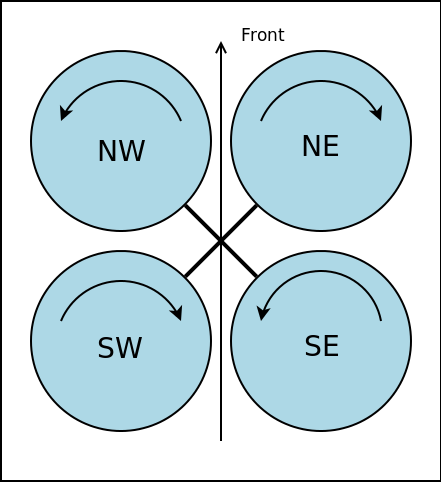
\includegraphics[width=5cm]{img/drehrichtung}
	\caption{Drehrichtung der Rotoren}
	\label{drehrichtung}

\end{figure}


\subsubsection{Flight Control}

Als FlightControl-Board verwenden wir ein Board vom Typ Paparazzi-Lia, auf dem bereits ein 10-DOM Lagesensor (IMU) integriert ist und auf dem die Paparazzi-Firmware läuft. Hier werden sowohl die Low-Level-Lageregelung als auch logisch höhere Funktionen wie Navigation umgesetzt und alle Aktuatoren und Sensoren angeschlossen.

\subsubsection{Sonar}
Die Sonarsensoren sind neben der IMU die wichtigsten Sensoren. Die Lagesensoren sind über I$^2$C an die Flightcontrol angebunden.
Die I$^2$C-Adressen der Sonarsensoren sind 0x71 bis 0x74, wobei 0x71 die Adresse des vorderen Sensors ist und im Uhrzeigersinn nummeriert wird.

Der Code für die Sensortreiber befindet sich in \path{sw/airborne/modules/sonar/sonar_array.c}.

\subsubsection{Farbsensor}
Der Farbsensor ist genau wie die Sonarsensoren per I$^2$C angebunden. Ein Treiber muss noch geschrieben werden\footnote{Zur Orientierung kann der Treiber für die Sonarsensoren genutzt werden.}.


\subsubsection{Bluetooth}
Bluetooth wird zum Empfang der Telemetriedaten und zur Steuerung des Autopiloten\footnote{Es geht als nicht um Manuellen Flug, sondern um Kommandos wie "Starten, Landen, Wegpunkt anfliegen etc.} genutzt.
Um Bluetooth nutzen zu können muss der Quadrocopter mit dem Rechner mit der Bodenstation gepairt werden – das ist leider bei jedem Start von neuem Notwendig, obwohl der Bluetoothstandart auch automatisches Pairing vorsieht.
\emph{Die PIN zum Pairing ist 1234.}


\subsection{Fernbedienung}
Die Fernbedienung dient zur manuellen Steuerung des Quadrocopters und zum Umschalten der Autopiloten-Modi.

\subsubsection{Manuelle Steuerung}
Der Wichtigste Schalter ist open Rechts: Der Kill-Schalter. Dieser Schalter funktioniert quasi als Not-Aus – alle Motoren werden sofort ausgeschalten.
Zum Losfliegen muss dieser Schalter deaktiviert werden.
Wichtig sind außerdem die beiden Steuerknüppel der Fernbedienung: Links ist Schub und Yaw, rechts Pitch und Roll.

\subsubsection{Autopiloten-Modi}
Mit dem drei Wege-Schalter oben rechts an der Fernbedienung (neben dem Kill-Schalter) kann der Modus des Autopiloten gewechselt werden.
Momentan sollten die Stellung unten – \enquote{Attitude Mode} zum manuellen Fliegen mit Fernsteuerung und die Stellung oben – \enquote{Nav Mode} zum autonomen Flug nach \enquote{flight-plan}.
Im Autopilotmodus wird je nach Einstellung der Schub durch den Schubhebel an der Fernsteuerung limitiert. \emph{Schaltet man wieder auf manuellen Modus um, versucht der Quadrocopter sofort diese Obergrenze als aktuellen Schub umzuseten!}
